% ============================================================
% Oppgave 4
% ============================================================

\hypertarget{oppgave4}{}
\section*{Oppgave 4}
\addcontentsline{toc}{section}{Oppgave 4}
Filteret har nullpunktene:
\[
z_1=-1,
\qquad
z_2=-2
\]
og en dobbeltpol i:
\[
p_1=p_2=0.8
\]
\subsection*{a)}
Systemfunksjonen kan bygges direkte fra nullpunktene og polene:
\[
H(z)
=
\frac{(z+1)(z+2)}
{(z-0.8)^2}
\]
Telleren blir:
\[
(z+1)(z+2)
=
z^2+3z+2
\]
Nevneren blir:
\[
(z-0.8)^2
=
z^2-1.6z+0.64
\]
Systemfunksjonen er derfor:
\[
\boxed{
H(z)
=
\frac{z^2+3z+2}
{z^2-1.6z+0.64}
}
\]
Ved å dividere teller og nevner med $z^2$ får vi:
\[
H(z)
=
\frac{1+3z^{-1}+2z^{-2}}
{1-1.6z^{-1}+0.64z^{-2}}
\]
\subsection*{b)}
Fra:
\[
H(z)
=
\frac{Y(z)}{X(z)}
=
\frac{1+3z^{-1}+2z^{-2}}
{1-1.6z^{-1}+0.64z^{-2}}
\]
får vi:
\[
Y(z)
\left(
1-1.6z^{-1}+0.64z^{-2}
\right)
=
X(z)
\left(
1+3z^{-1}+2z^{-2}
\right)
\]
I tidsdomenet blir dette:
\[
y[n]
-
1.6y[n-1]
+
0.64y[n-2]
=
x[n]
+
3x[n-1]
+
2x[n-2]
\]
Løser vi med hensyn på $y[n]$ får vi differensligningen:
\[
\boxed{
y[n]
=
1.6y[n-1]
-
0.64y[n-2]
+
x[n]
+
3x[n-1]
+
2x[n-2]
}
\]
Filteret har både forsinkede inngangsverdier og forsinkede
utgangsverdier. Det er derfor et rekursivt IIR-filter. Figuren under viser strukturen til filteret.
\begin{figure}[H]
\centering
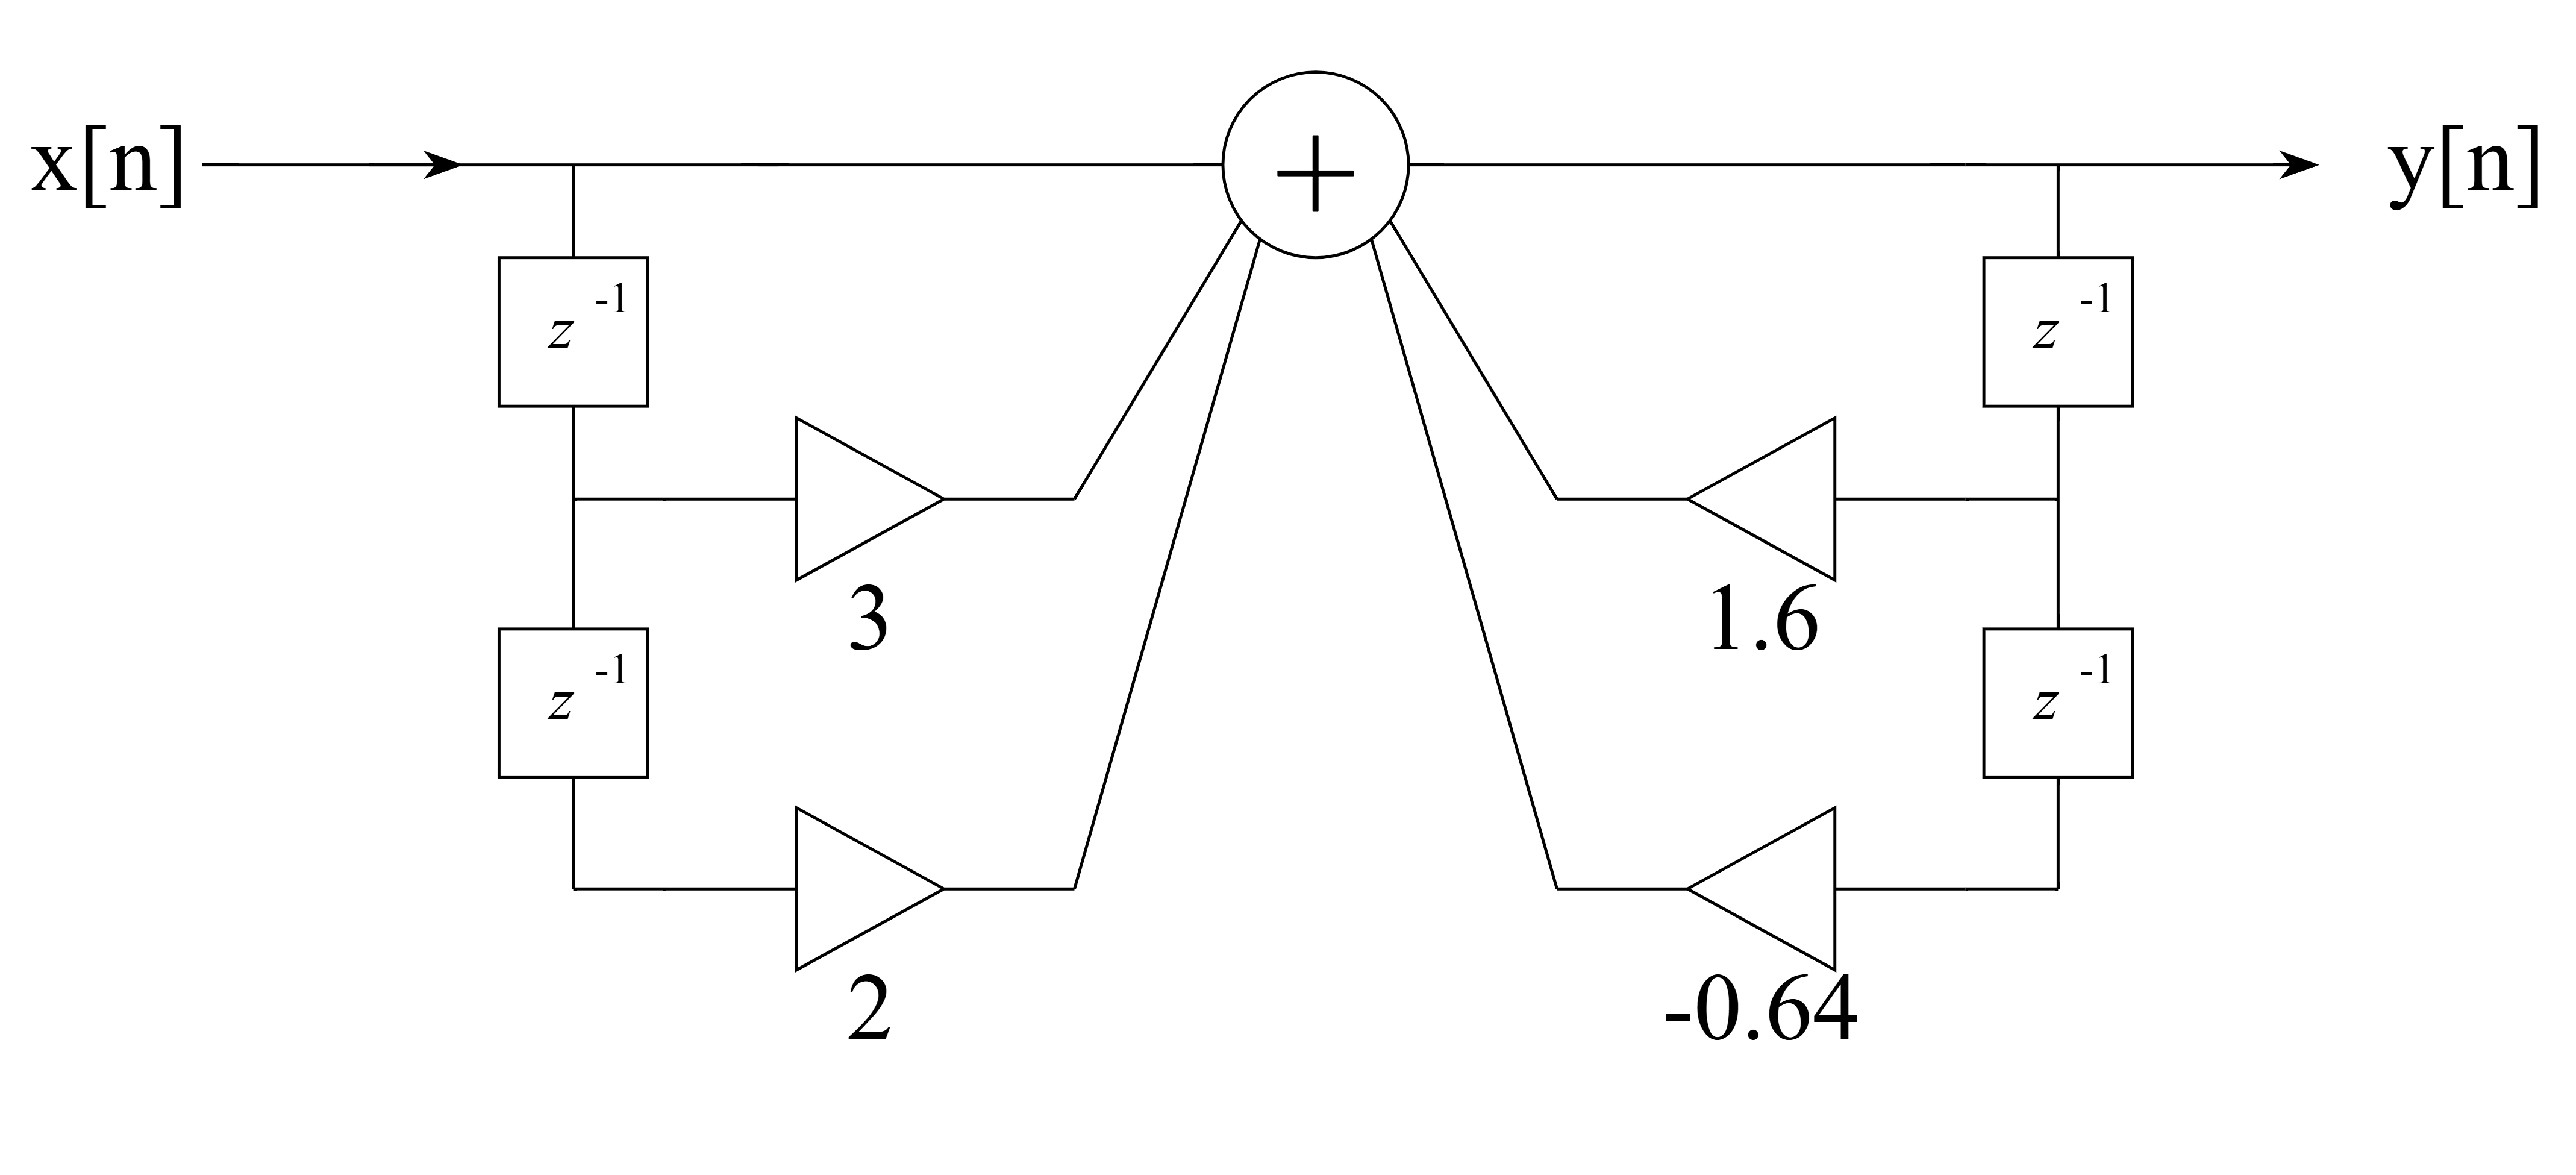
\includegraphics[width=1\textwidth]{Media/iir1.png}
\caption{Strukturdiagram for det rekursive IIR-filteret.}
\end{figure}
\subsection*{c)}
Innsignalet er:
\[
x[n]=\{2,3,-1\}
\]
og vi antar at:
\[
x[n]=0
\]
utenfor den oppgitte sekvensen og at filteret starter i ro:
\[
y[-1]=y[-2]=0
\]
Differensligningen brukes for $n=0,\ldots,6$:
\[
\begin{array}{c|c|c}
n & x[n] & y[n] \\
\hline
0 & 2  & 2.000000 \\
1 & 3  & 12.200000 \\
2 & -1 & 30.240000 \\
3 & 0  & 43.576000 \\
4 & 0  & 48.368000 \\
5 & 0  & 49.500160 \\
6 & 0  & 48.244736
\end{array}
\]
\subsection*{d)}
Et kausalt digitalt IIR-filter er stabilt dersom alle polene
ligger innenfor enhetssirkelen:
\[
|p|<1
\]
Begge polene ligger i:
\[
p=0.8
\]
og dermed:
\[
|0.8|<1
\]
Filteret er derfor stabilt.
\subsection*{e)}
Systemfunksjonen kan skrives som:
\[
H(z)
=
\frac{1+3z^{-1}+2z^{-2}}
{(1-0.8z^{-1})^2}
\]
Ved delbrøkoppspalting får vi:
\[
H(z)
=
3.125
-
\frac{10}{1-0.8z^{-1}}
+
\frac{7.875}{(1-0.8z^{-1})^2}
\]
Vi bruker transformparene:
\[
\frac{1}{1-az^{-1}}
\longleftrightarrow
a^n u[n]
\]
og:
\[
\frac{1}{(1-az^{-1})^2}
\longleftrightarrow
(n+1)a^n u[n]
\]
Impulsresponsen blir dermed:
\[
h[n]
=
3.125\delta[n]
-
10(0.8)^n u[n]
+
7.875(n+1)(0.8)^n u[n]
\]
Dette kan også skrives som:
\[
\boxed{
h[n]
=
3.125\delta[n]
+
(7.875n-2.125)(0.8)^n u[n]
}
\]
Siden faktoren $(0.8)^n$ går mot null når $n$ øker, dør
impulsresponsen etter hvert ut.


\subsection*{f)}
Man kan ikke generelt avgjøre stabiliteten bare ved å se på
størrelsen til koeffisientene i differensligningen.
Koeffisientene bestemmer plasseringen til polene, men det er
polplasseringen som avgjør stabiliteten.
For et kausalt digitalt filter er BIBO-stabilitet oppnådd når alle polene ligger innenfor enhetssirkelen, altså:
\[
\boxed{
|p_k|<1
\quad
\text{for alle poler}
}
\]
Hvis en eller flere poler ligger på eller utenfor enhetssirkelen, er filteret ikke BIBO-stabilt, og et begrenset inngangssignal kan gi et ubegrenset utgangssignal.